% ticks=none with longer tick lengths elsewhere; second axis with tickwidth/subtickwidth and ticks on the upper sides.
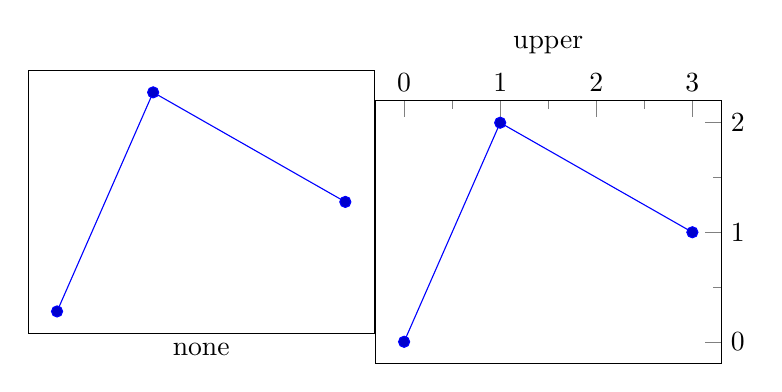
\begin{tikzpicture}
\begin{axis}[name=a, ticks=none, width=170pt, height=140pt, xlabel={none}]
  \addplot coordinates {(0,0) (1,2) (3,1)};
\end{axis}
\begin{axis}[at={(a.outer south east)}, anchor=outer south west, width=170pt, height=140pt, tickwidth=6pt, subtickwidth=3pt, minor tick num=1, xtick pos=upper, ytick pos=right, xlabel={upper}]
  \addplot coordinates {(0,0) (1,2) (3,1)};
\end{axis}
\end{tikzpicture}
